% !Mode:: "TeX:UTF-8"
\chapter{SLAM: Present and Future}
\label{cpt:14}
\begin{mdframed}  
	\textbf{Goal of Study}
	\begin{enumerate}[labelindent=0em,leftmargin=1.5em]
		\item Understand the classic SLAM implementation scheme.
		\item Through experiments, compare the similarities and differences of various SLAM solutions.
		\item Explore the future development direction of SLAM.
	\end{enumerate}
\end{mdframed}

The previous chapters introduce the widely used SLAM pipelines, which are the conclusion of decades of researches. At present, in addition to the theoretical frameworks, we can also find many excellent open-source SLAM solutions. However, since most of their implementations are more complicated and not suitable for beginners' hands-on materials, we put them at the end of the book to introduce them. I believe that readers should be able to understand the basic principles by reading the previous content.

\newpage
\section{Open-source Implementations}
This lecture is a summary of the book. We will take readers to see how far the existing SLAM solutions have gone. In particular, we focus on solutions that provide open-source implementations. In the early days, it is not easy to see open-source solutions. Usually, the theories introduced in the research paper only account for 20\% of the content, and the other 80\% are in the code, which is not mentioned. These researchers' selfless dedication has promoted the entire SLAM community's rapid advancement and enabled subsequent researchers to have a higher starting point. Before we start to do SLAM, we should have an in-depth understanding of similar solutions and then conduct our own research.

The first half of this lecture will lead the readers to take a tour of the current visual SLAM program and comment on its historical status, advantages and disadvantages. \autoref{table:opensource-slam}~ lists some popular open-source SLAM solutions. Readers can choose the interesting solutions for research and experiments \footnote{The book was basically written in 2016, so I did not list the newer systems after 2016.}. We only selected a part of the representative ones due to space limitations, which is certainly not complete. We will explore some possible future development directions in the second half and provide some current research results.

\begin{table}[!h]
	\small
	\caption{Open source SLAM systems}
	\label{table:opensource-slam}
	\begin{threeparttable}
	\begin{tabular}{c|c|c}%{@{}c|c|X@{}}
		\hline\hline
		Name & Sensors\tnote{*} & URL \\
		\hline
		MonoSLAM &  M & \url{https://github.com/hanmekim/SceneLib2}  \\ 
		PTAM & M & \url{http://www.robots.ox.ac.uk/~gk/PTAM/} \\ 
		ORB-SLAM & M/S/R & \url{http://webdiis.unizar.es/~raulmur/orbslam/} \\ 
		LSD-SLAM & M & \url{http://vision.in.tum.de/research/vslam/lsdslam} \\
		SVO & M & \url{https://github.com/uzh-rpg/rpg_svo} \\ 
		DTAM & R & \url{https://github.com/anuranbaka/OpenDTAM} \\ 
		DVO & R & \url{https://github.com/tum-vision/dvo_slam} \\ 
		DSO & M & \url{https://github.com/JakobEngel/dso} \\
		VINS & M+IMU & \url{https://github.com/HKUST-Aerial-Robotics/VINS-Mono} \\
		RTAB-MAP & S/R & \url{https://github.com/introlab/rtabmap} \\ 
		RGBD-SLAM-V2 & R & \url{https://github.com/felixendres/rgbdslam_v2} \\ 
		Elastic Fusion & R & \url{https://github.com/mp3guy/ElasticFusion} \\ 
		Hector SLAM & L & \url{http://wiki.ros.org/hector_slam} \\ 
		GMapping & L & \url{http://wiki.ros.org/gmapping} \\ 
		OKVIS & M/S+IMU & \url{https://github.com/ethz-asl/okvis} \\ 
		ROVIO & M+IMU & \url{https://github.com/ethz-asl/rovio} \\ 
		\hline\hline
	\end{tabular}

	\begin{tablenotes}
		\footnotesize
		\item [*] M=Monocular, S=Stereo, R=RGB-D, L=Lidar.
	\end{tablenotes}
	\end{threeparttable}
\end{table}

\subsection{MonoSLAM}
When talking about visual SLAM, the first thing that many researchers think of is A. J. Davison's monocular SLAM {\cite{Davison2007,Davison2003}}. Professor Davison is a pioneer in this area. He proposed MonoSLAM in 2007 as the first real-time monocular visual SLAM system {\cite{Davison2007}}, which is considered the birthplace of many works. MonoSLAM uses the extended Kalman filter as the backend to track very sparse feature points on the frontend. Since EKF occupies a prominent dominant position in early SLAM, MonoSLAM is also based on EKF, using the current state of the camera and all landmark points as the state quantity, and updating the mean and covariance of the states.

\autoref{fig:mono-slam}~ shows the snapshot of MonoSLAM. The monocular camera tracks very sparse feature points in an image using active tracking technology. In EKF, each feature's position obeys the Gaussian distribution, so we can express its mean value and uncertainty as an ellipsoid. In the right half of the picture, we can find some small ellipsoids distributed in 3D space. If the ellipsoid looks long in a specific direction, the landmark corresponding to it is more uncertain in that direction. We can imagine that if a feature point converges, we should see it change from a very long ellipsoid (initially very uncertain in the $Z$ axis of the camera system) to a small point.

\begin{figure}[!htp]
	\centering
	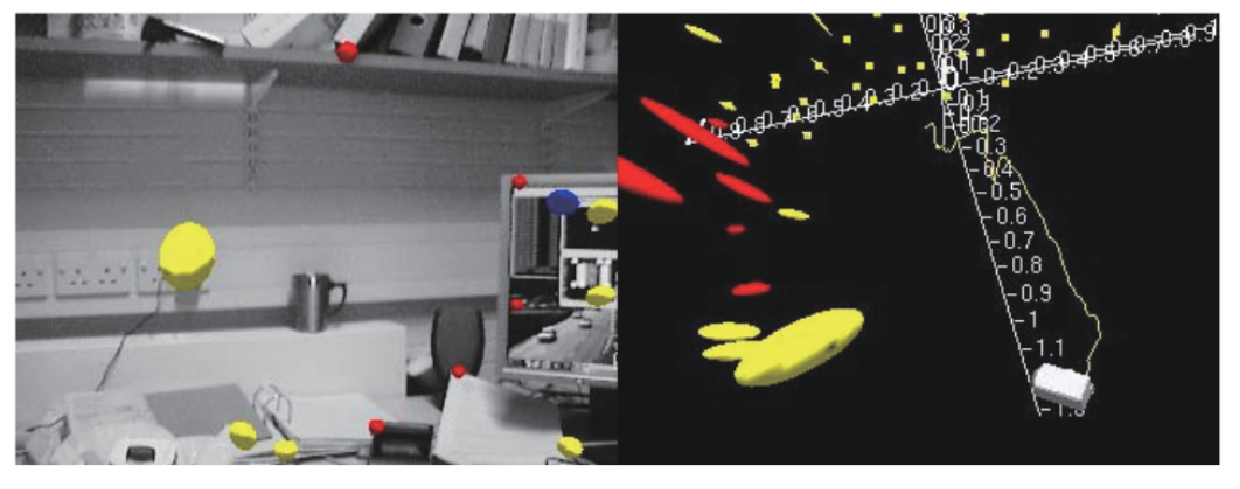
\includegraphics[width=1.0\textwidth]{past-and-future/mono-slam.pdf}
	\caption{Snapshot of MonoSLAM. Left: the tracked features. Right: the map point in 3D space.}
	\label{fig:mono-slam}
\end{figure}

This approach seems to have many drawbacks today. Still, it was already a milestone work at that time because most of the previous visual SLAM systems could not run online. The advancement of CPU performance and sparse bundle adjustment combined to make a SLAM system run online. From a modern point of view, MonoSLAM has drawbacks such as the small scenarios, limited number of landmarks, and sparse feature points that are very easy to lose. Its maintaining work has also been stopped and replaced by more advanced theories and programming tools. But this does not prevent us from understanding and respecting the work of our predecessors.

\subsection{PTAM}
In 2007, Klein's team proposed PTAM (Parallel Tracking and Mapping) {\cite{Klein2007}}, which is also an important event in the development of visual SLAM. The important significance of PTAM lies in the following two points:
\begin{enumerate}
	\item PTAM proposed and realized the parallelization of the tracking and mapping process. Most people think it is clear that the tracking part needs to respond to image data in real-time, and the optimization does not need to be calculated in real-time. Backend optimization can be done slowly in the background, and then thread synchronization can be performed when necessary. This is the first time the concept of front and backends have been distinguished in visual SLAM, leading to the structure of many later visual SLAM systems (most of the SLAMs we see now are divided into front and backends).
	\item PTAM is the first real-time solution that uses nonlinear optimization instead of traditional filters in the backend. It introduces the keyframe mechanism: we don't need to process each image carefully but string together several key images and optimize its trajectory and map. Early SLAM mostly used EKF filters or their variants. After PTAM, visual SLAM research gradually turned to the backend dominated by nonlinear optimization. 
	
	PTAM is also an augmented reality software that demonstrates promising AR effects (as shown in \autoref{fig:ptam}). According to the camera pose estimated by PTAM, we can place a virtual object on a virtual plane, which looks like it is in a real scene.
\end{enumerate}

\begin{figure}[!ht]
	\centering
	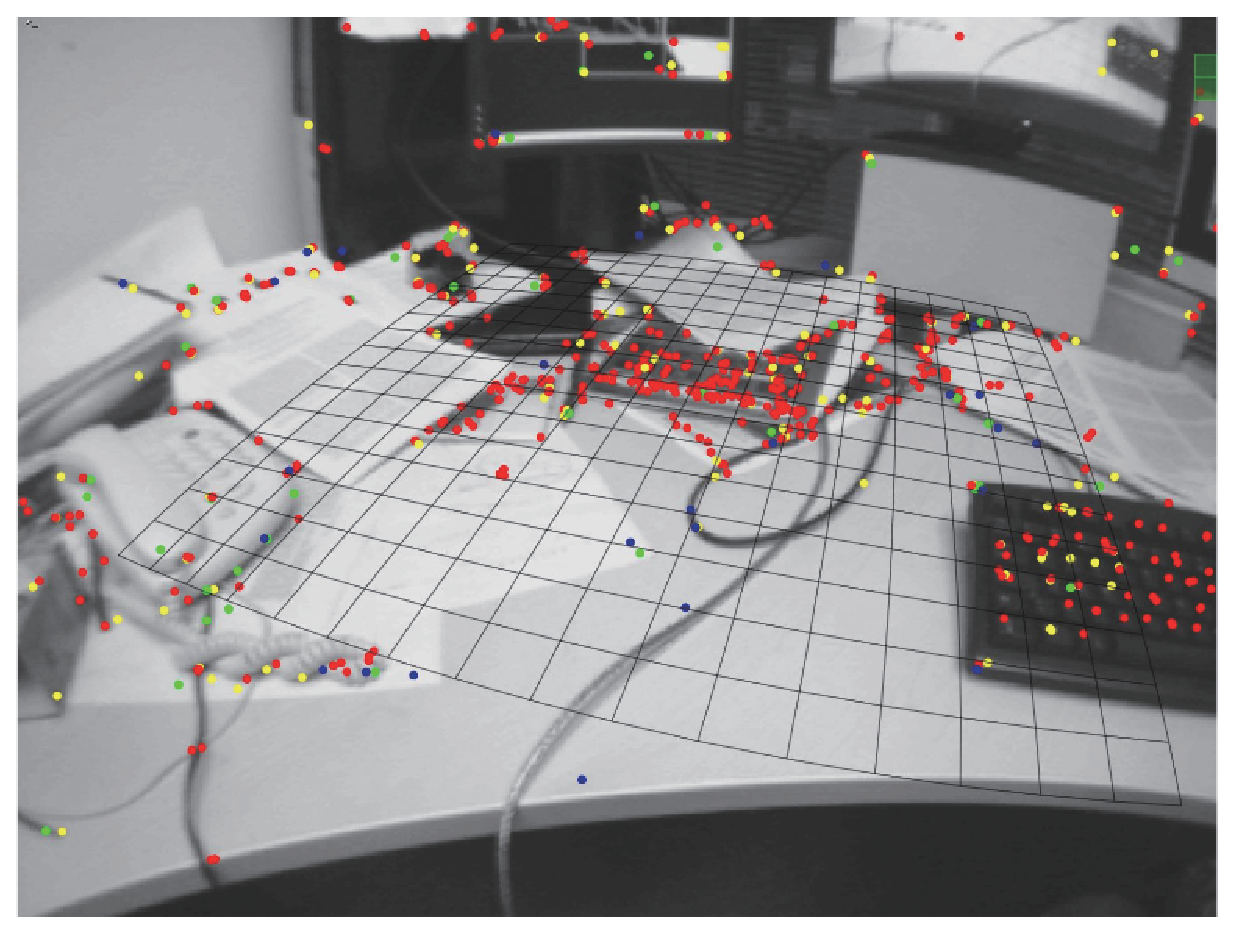
\includegraphics[width=1.0\textwidth]{past-and-future/ptam}
	\caption{Screenshot of PTAM demo. It can provide not only real-time SLAM functions but also superimpose virtual objects on a virtual plane.}
	\label{fig:ptam}
\end{figure}

However, from a modern perspective, PTAM can be regarded as one of the early SLAM work combined with AR. Like many previous works, there are apparent defects: the scene is small, tracking is easy to lose, and so on. These were improved in the follow-up systems.

\subsection{ORB-SLAM Series} 
After introducing several historical solutions, let's look at some modern SLAM systems. ORB-SLAM is a very famous \textsuperscript{\cite{Mur-Artal2015}} among the successors of PTAM (see \autoref{fig:orb-slam}). It was proposed in 2015 and is one of the most complete and easy-to-use systems in modern SLAM systems (if not the most complete and easy-to-use). ORB-SLAM is a peak of the mainstream feature-based open-source SLAM. Compared with previous work, ORB-SLAM has the following obvious advantages:

\begin{figure}[!ht]
	\centering
	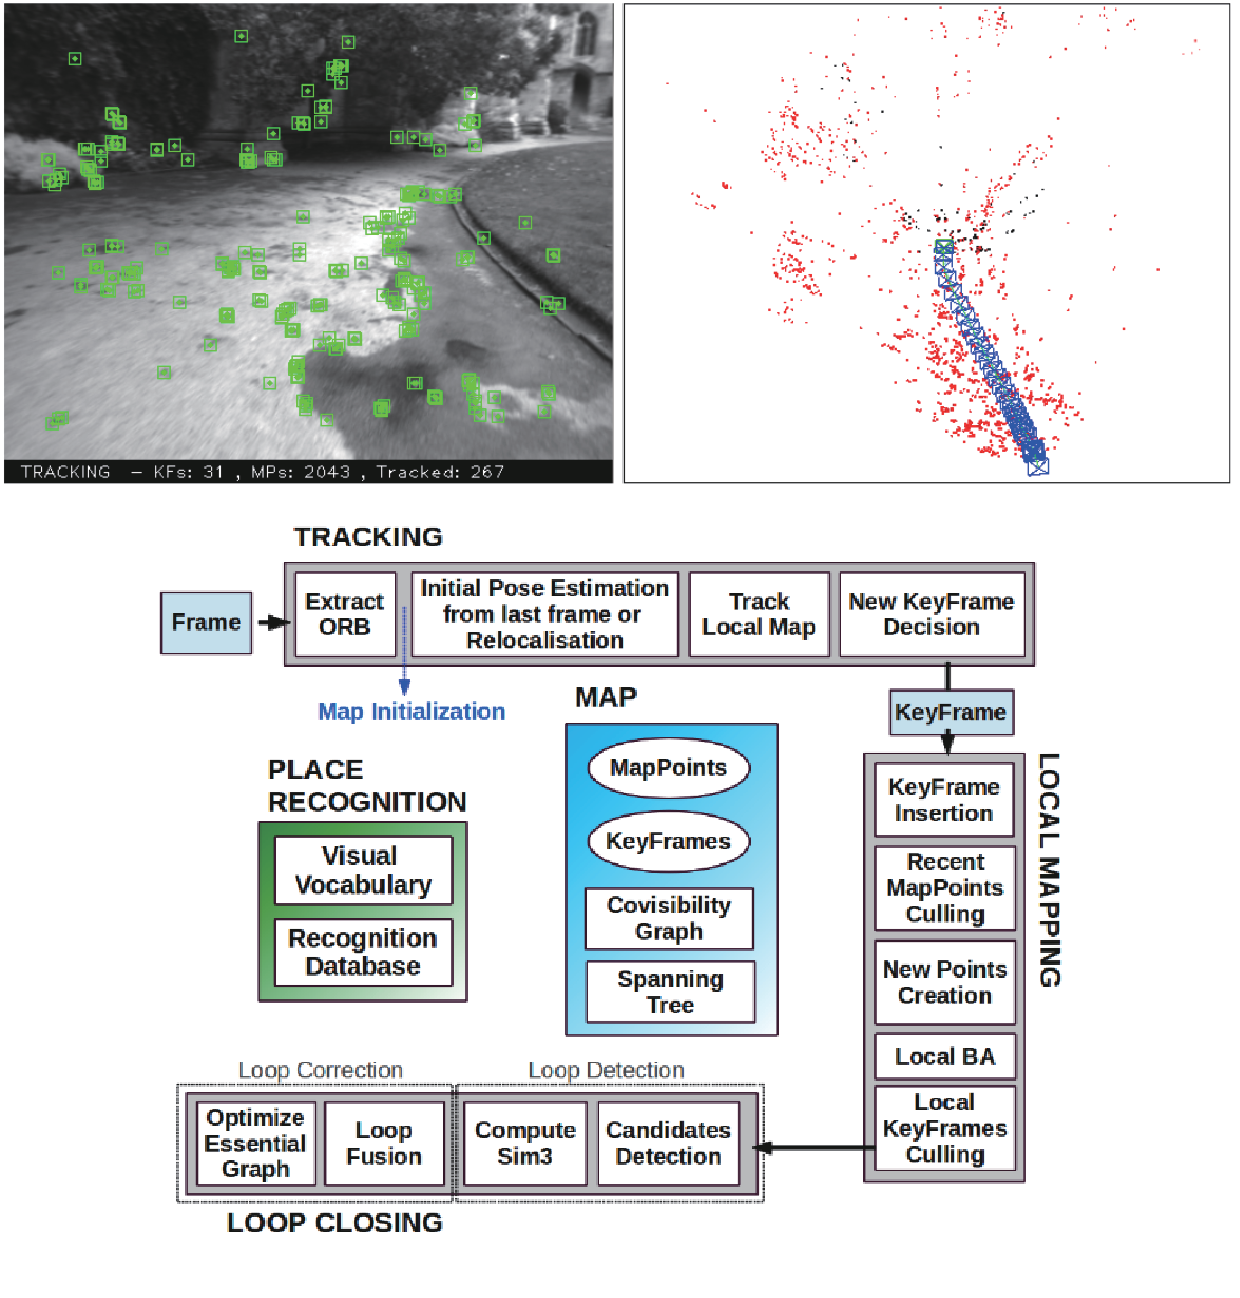
\includegraphics[width=1.0\textwidth]{past-and-future/orb-slam}
	\caption{ORB-SLAM running screenshot. The left side is the image and the tracked feature points, and the right side is the camera trajectory and the modeled feature point map. Below is the three-thread framework.}
	\label{fig:orb-slam}
\end{figure}

\begin{enumerate}
	\item It supports various sensor settings: monocular, binocular, and RGB-D. For most of the sensors, it is almost possible to test it on ORB-SLAM. It has good versatility.
	\item The entire system is calculated with ORB features, including the ORB dictionary for visual odometry and loop detection. It reflects that the ORB feature is an excellent compromise between the computing platform's efficiency and accuracy at this stage. ORB is not as time-consuming as SIFT or SURF and can be calculated in real-time on the CPU; compared to simple corner features such as Harris corners, it has good rotation and scaling invariance. Also, ORB provides descriptors that enable us to perform loop detection and relocation in a large range of motion.
	\item ORB's loop detection is its highlight. The excellent loop closure detection algorithm ensures that ORB-SLAM effectively prevents accumulated errors and can be quickly retrieved after being lost. Many existing SLAM systems are not perfect in the relocalization point. For this reason, ORB-SLAM needs to load a large ORB dictionary file.
	\item ORB-SLAM innovatively uses the three threads structure in SLAM: Tracking thread for real-time tracking of feature points, optimization thread for local bundle adjustment (co-visibility Graph, commonly known as the \textit{small graph}), and global pose graph optimization thread (essential graph, known as the \textit{big graph}). The tracking thread is responsible for extracting ORB feature points for each new image, comparing it with the most recent keyframe, calculating the feature points' location, and roughly estimating the camera pose. The small graph solves a local bundle adjustment problem, including the feature points in the local space and the camera pose. This thread is responsible for refining camera poses and spatial locations of feature points. The tracking and local mapping threads construct good visual odometry. The third thread, the big graph thread, performs loop detection on the global map and keyframes to eliminate accumulated errors. 
	
	Following the two-thread structure of PTAM, the three-thread design of ORB-SLAM has achieved excellent tracking and mapping effects, ensuring the global consistency of the trajectory and the map. This three-thread structure will also be accepted and adopted by subsequent researchers.
	\item ORB-SLAM has carried out many optimizations around feature points. For example, based on OpenCV feature extraction, ORB-SLAM uniforms the distribution of image features. When optimizing the pose, a four-iteration optimization routine is used to obtain better matches. A more relaxed keyframe selection strategy than PTAM is also used. These small improvements make ORB-SLAM far more robust than other solutions: even for poor scenarios and poor calibration parameters, ORB-SLAM can work smoothly.
\end{enumerate}

The advantages mentioned above make ORB-SLAM reach the state-of-the-art open-source visual SLAM system. Many research works use ORB-SLAM as the standard or follow-up development. Its code is known for being clear and easy to read with sufficient annotations, being friendly to later researchers. 

Of course, ORB-SLAM also has some shortcomings. Since the entire SLAM system uses feature points for calculation, we must detect the ORB feature for each image, which is very time-consuming. ORB-SLAM's three-thread structure also brings a heavier burden to the CPU, making it only able to operate in real-time on the current PC's CPU. It is not easy to transform into embedded devices. Secondly, the ORB-SLAM map consists of sparse feature points. But it does not implement the storage and relocation functions after closing the SLAM software (although it is not difficult in terms of implementation). According to chapter \ref{cpt:12}, the sparse feature point map can only meet our localization needs but cannot satisfy navigation, obstacle avoidance, interaction, or other requirements. However, if we only use ORB-SLAM to deal with the localization problem, it seems a bit too heavyweight. In contrast, some other programs provide a more lightweight localization, allowing us to run SLAM on low-level processors.

\subsection{LSD-SLAM}
LSD-SLAM (Large Scale Direct monocular SLAM) is a SLAM work {\cite{Engel2013, Engel2014}} proposed by J. Engel et al. in 2014. Analogous to ORB-SLAM to feature points, LSD-SLAM marks the direct method's successful application in monocular SLAM. The core contribution of LSD-SLAM is to apply the direct method to semi-dense monocular SLAM. It does not need to calculate the features but can also construct a semi-dense map. The semi-dense means estimating the pixel position with an obvious gradient. Its main advantages are as follows:

\begin{enumerate}
	\item The direct method of LSD-SLAM is for pixels. The authors creatively proposed the relationship between pixel gradient and the direct method. And also, they note the angular relationship between pixel gradient and epipolar direction in dense reconstruction. These are discussed in lecture \ref{cpt:8} and \ref{cpt:12} in this book. However, LSD-SLAM performs semi-dense tracking on monocular images, and the implementation detail is more complicated than the routines in this book.
	\item LSD-SLAM realizes the semi-dense reconstruction on CPU, which is rarely seen in previous schemes. The method based on feature points can only be sparse, and most of the dense reconstruction schemes use RGB-D sensors or use GPU to build dense maps {\cite{Kerl2013}}. 
	\item The semi-dense tracking of LSD-SLAM uses some subtle tricks to ensure the tracking's real-time efficiency and stability. For example, LSD-SLAM does not use a single-pixel or image block for epipolar searching but takes five points on the epipolar line at equal distances to measure its SSD. In the depth estimation, LSD-SLAM first initializes the depth with random numbers and then normalizes the depth estimation after converges. When measuring the depth uncertainty, it considers the triangle's geometric relationship and the angle between the epipolar line and the image gradient. The loop closure thread uses the similarity transformation group $\mathrm{SE}(3)$ to express the scale explicitly, which can be used to reduce the scale drift in monocular SLAM.
\end{enumerate}

\autoref{fig:lsd-slam}~ shows a snapshot of the LSD-SLAM. We can observe how this semi-dense map is a form between the sparse map and the dense map. The semi-dense map models the parts with apparent gradients in the grayscale image. A large part of the map is displayed on the edges or textured parts of the object. LSD-SLAM tracks them and establishes the keyframes, and finally optimizes to get such a map. It seems that it has more information than a sparse map, but it does not have complete surfaces like a dense map (dense maps are generally considered to be unable to achieve real-time performance with CPU alone).

\begin{figure}[!ht]
	\centering
	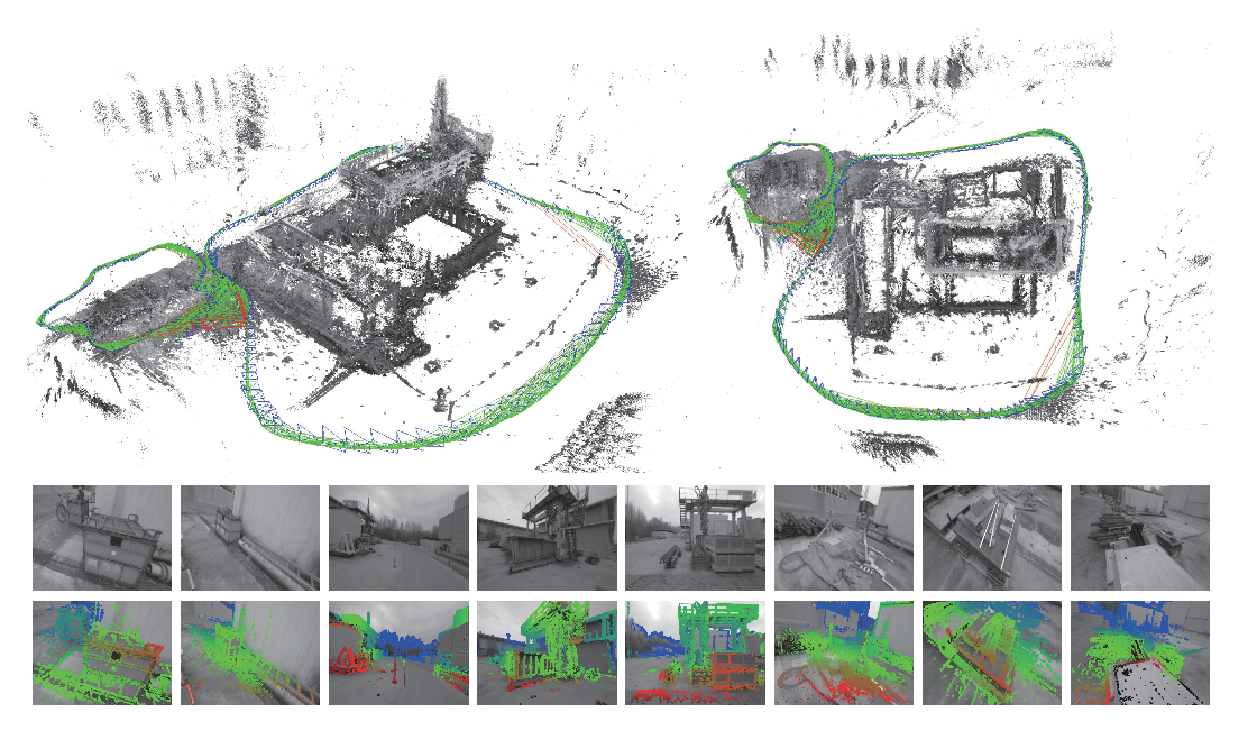
\includegraphics[width=1.0\textwidth]{past-and-future/lsd-slam}
	\caption{Snapshots of LSD-SLAM. The upper part is the estimated trajectory and map, and the lower part is the reconstructed part of the image, that is, the part with better pixel gradients.}
	\label{fig:lsd-slam}
\end{figure}

Since LSD-SLAM uses the direct tracking method, it has both the direct method's advantages and disadvantages. For example, LSD-SLAM is very sensitive to camera intrinsics and exposure time and is easily lost when the camera moves quickly. Also, in the loop detection part, LSD-SLAM still relies on the feature point method for loop detection and has not entirely eliminated the calculation of feature points.

\subsection{SVO}
SVO is the abbreviation of Semi-direct Visual Odometry \cite{Forster2014}. It is visual odometry based on the sparse direct method proposed by Forster et al. in 2014. According to the author's name, it should be called the ``semi-direct'' method, but according to the conceptual framework of this book, it may be better to call it the ``sparse direct method''. The meaning of semi-direct in the original text refers to the mixed-use of feature points and direct methods: SVO tracks some key points (corner points, no descriptors), and then, like the direct method, uses the information of these key points to estimate camera movement and the map point's position (as shown in \autoref{fig:svo}). In the implementation, SVO uses small blocks of $4\times4$ around the key points for block matching to estimate the camera's motion.

Compared with other programs, SVO's most significant advantage is high-speed. Due to the use of the sparse direct method, it does not have to laboriously calculate the descriptor, nor does it need to process as much information as dense and semi-dense approaches. So, it can achieve real-time performance even on low-level computing platforms. On PC platforms, it can reach a speed of more than 100 frames per second. In the subsequent SVO 2.0, the speed has reached an astonishing 400 frames per second. This makes SVO very suitable for scenarios with limited computing resources, such as the localization of drones and handheld AR/VR devices. UAV is also the target application platform for the author to develop SVO.

\begin{figure}[!htp]
	\centering
	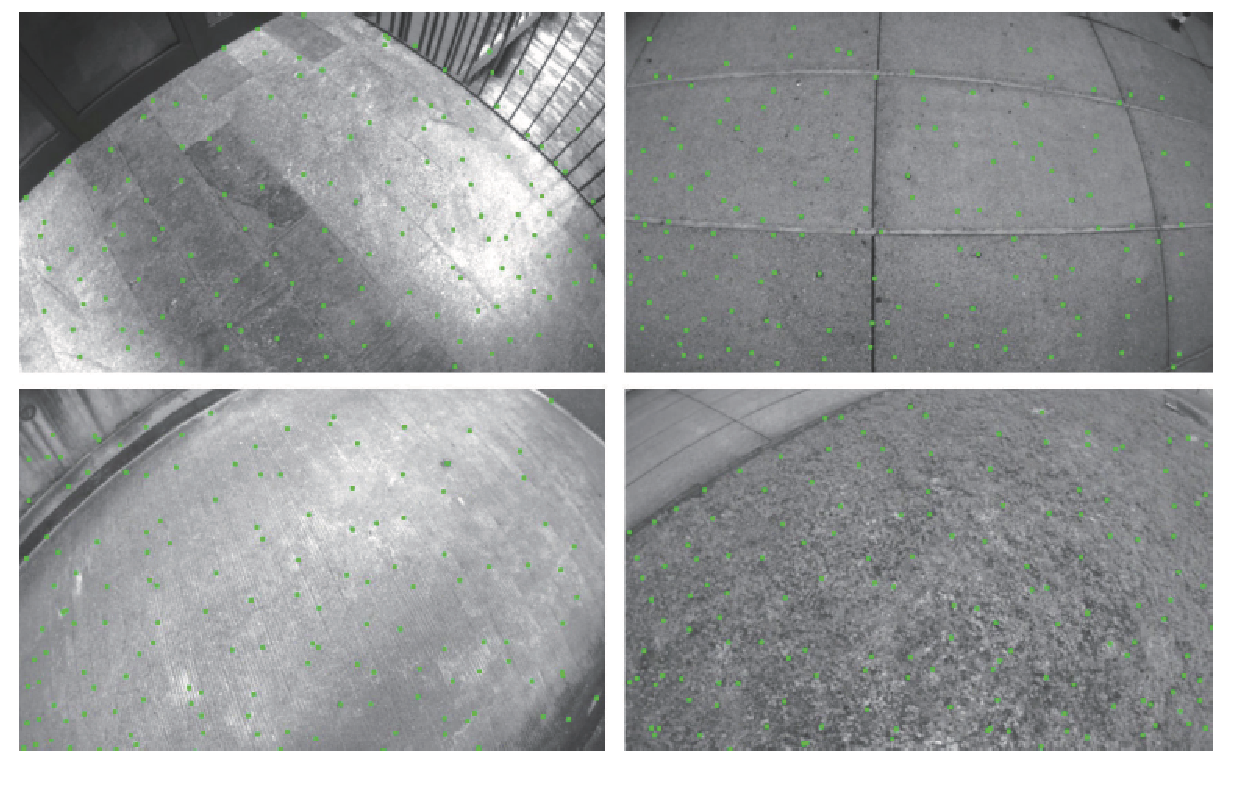
\includegraphics[width=1.0\textwidth]{past-and-future/svo}
	\caption{Features tracked by SVO.}
	\label{fig:svo}
\end{figure}

Another SVO innovation is that it puts forward the concept of depth filter and derives a depth filter based on uniform-Gaussian mixture distribution. This is mentioned in lecture \ref{cpt:12} of this book, but since the principle is more complicated, we did not explain it in detail. SVO uses this filter to estimate the key points' depth and uses the inverse depth parameterization to better calculate feature points' position.

SVO's code is clear and easy to read, which is very suitable for readers to analyze as the first SLAM example. However, the open-source version of SVO also has some problems:
\begin{enumerate}
	\item Since the target application platform is the drone's top-down camera, the object in its field of view is mainly the ground. The camera's movement is mostly horizontal rotation and up-and-down movement. Many SVO details are designed around this application, making its performance not very good for front-seeing cameras. For example, SVO uses the decomposition of the $\mathbf{H}$ matrix instead of the traditional $\mathbf{F}$ or $\mathbf{E}$ matrix during monocular initialization, which requires the assumption that the feature points are on the plane. This assumption is correct for a top-down camera, but it is usually not valid for a head-up camera. When SVO selects a keyframe, it uses the translation amount to determine a new keyframe without considering the rotation amount. This is also effective in the drone's top view configuration, but it is easy to lose in the head-up camera. Therefore, if readers want to use SVO in a head-up camera, some modification is needed.
	\item SVO discards the backend optimization and loop closure detection part for speed and lightweight. And it basically has no mapping functions. This means that SVO pose estimation must have accumulative errors, and it is not easy to relocate after loss (because there is no descriptor for loop detection). Therefore, we call it a VO, not a complete SLAM.
\end{enumerate}

\subsection{RTAB-MAP}
After introducing several monocular SLAM solutions, let's look at some SLAM solutions on RGB-D sensors. Compared with monocular and binocular cameras, the RGB-D SLAM principle is much more straightforward (though not necessarily in implementation). It can build dense maps in real-time on the CPU.

RTAB-MAP (Real-Time Appearance-Based Mapping) {\cite{Labbe2014}} is a classic scheme in RGB-D SLAM. It implements everything that should be included in RGB-D SLAM: feature-based visual odometry, bag-of-words-based loop detection, backend pose map optimization, and point cloud and triangular mesh maps. Therefore, RTAB-MAP provides a complete (but somewhat huge) RGB-D SLAM solution. At present, we can obtain the binary program directly from ROS. In addition, the App can also be used on Google Project Tango (as shown in \autoref{fig:rtabmap}~).

\begin{figure}[!ht]
	\centering
	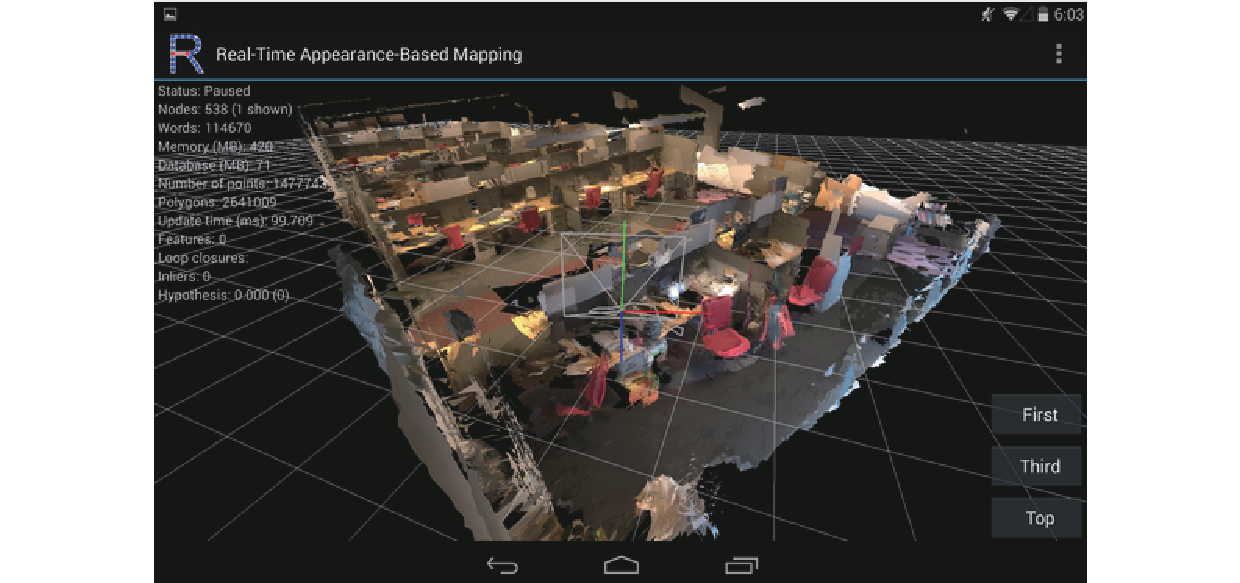
\includegraphics[width=1.0\textwidth]{past-and-future/rtabmap}
	\caption{RTAB-MAP in Google Project Tango.}
	\label{fig:rtabmap}
\end{figure}

RTAB-MAP supports some common RGB-D and binocular sensors, such as Kinect, Xtion, etc., and provides real-time localization and mapping functions. However, due to the high integration level, it becomes difficult for other developers to carry out secondary development. RTAB-MAP is more suitable for SLAM applications than research use.

\subsection{Others}
In addition to these open source solutions, readers can also find many other studies on websites such as \url{openslam.org}, for example, DVO-SLAM {\cite{Kerl2013a}}, RGBD-SLAM-V2 {\cite{Endres2014}}, DSO  {\cite{Engel2016}}, and some Kinect Fusion related work, etc. With the development of the times, newer and better open-source SLAM works will also appear. Due to space limitations, we will not introduce them one by one here.

\section{SLAM in Future}
After studying the existing systems, let's discuss some future development directions \footnote{Well, this part is my personal understanding, which may not be completely correct.}. Generally speaking, SLAM's future development trend is divided into two categories: one is to develop towards lightweight and miniaturization so that SLAM can run well on small devices such as embedded or mobile phones, and then consider high-level applications that use it as the underlying function. After all, in most cases, our real goal is to realize the functions of robots and AR/VR devices, such as sports, navigation, teaching, and entertainment. SLAM is to provide its own pose estimation for upper-level applications. In these applications, we do not want SLAM to occupy many computing resources, so there is a solid demand for SLAM's miniaturization and lightweight. The second is to use high-performance computing equipment to realize precise 3D reconstruction and scene understanding. In these applications, our goal is to reconstruct the scene perfectly, and there are no restrictions on the portability of computing resources and equipment. Since GPU can be used, this direction and deep learning also have combination points.

\subsection{IMU Integrated VSLAM}
First, we want to talk about a direction with a strong application background: the visual-inertial navigation scheme. Whether in robots or hardware devices, we do not rely on one sensor but often have multiple sensors. Researchers in academia love the big clean problems, such as implementing visual SLAM with a single camera. But friends in the industry pay more attention to making algorithms more practical and face complex and corner-case scenarios. In this application context, vision and inertial integrated SLAM have become a hot spot.

The inertial sensor (IMU) can measure the angular velocity and acceleration of the sensor body, which is considered to be evidently complementary with the camera sensor and has the potential to obtain a more complete SLAM system after fusion {\cite{Gui2015}}. Why do we say that?

\begin{enumerate}
	\item IMU can measure angular velocity and acceleration, but these quantities have a noticeable drift, making the pose data obtained by the twice integration unreliable. For example, if we put the IMU on the table without moving, the post obtained by integrating its readings will drift far away in a short time. However, for fast movements, IMU can provide some better estimates than the camera. 
	
	When the movement is too fast, the rolling shutter camera will have a motion blur. The overlapping area between two frames is too small to perform any feature matching, so pure visual SLAM is very weak against the fast movement. With IMU, we can still maintain the pose estimation even when the camera images are invalid, which is not possible with pure visual SLAM.
	
	\item Compared with raw IMU integration, the camera data will basically not drift. If the camera is placed in place and fixed in a static scene, visual SLAM's pose estimation is also fixed. Therefore, the camera data can effectively estimate and correct the drift in the IMU reading so that the pose estimation after slow motion is still valid.
		
	\item When the image changes, we practically cannot know whether the camera has moved or the environmental objects have changed. In pure visual SLAM, it is difficult to deal with a large number of dynamic obstacles. But the IMU can feel its own motion. To some extent, VIO (Visual Inertial Odometry) can reduce the impact of dynamic objects.
\end{enumerate}

In summary, we see that IMU provides a better solution for fast motion, and the camera can solve the drift problem of IMU under slow motion. In this sense, the two are complementary.

\begin{figure}[!thp]
	\centering
	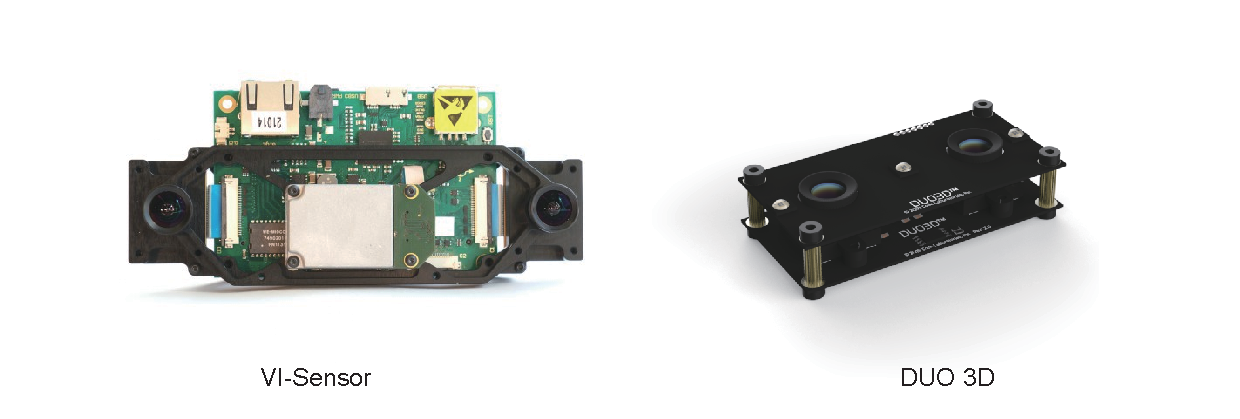
\includegraphics[width=1.0\textwidth]{past-and-future/visensor}
	\caption{More and more devices start to integrate IMU with cameras. }
	\label{fig:visensor}
\end{figure}

Although it sounds perfect, VIO is quite complicated, both in theory or practice. Its complexity mainly comes from the fact that IMU measures acceleration and angular velocity, so kinematic calculations have to be involved in the computation. At present, the VIO framework has been finalized into two categories: loosely coupled and tightly coupled {\cite{Martinelli2014}}. Loosely coupled means that the IMU and the camera perform their own motion estimation separately, and we merge their pose estimation results. Tightly coupled refers to combining the IMU state with the camera, jointly constructing the motion equation and observation equation, and then performing state estimation. This is very similar to the theory we introduced before. We can foresee that tightly coupled theory will also be divided into two directions: filtering-based and optimization-based. In terms of filtering, the traditional EKF {\cite{Bloesch2015}} and the improved MSCKF (Multi-State Constraint KF) {\cite{Li2013}} have achieved certain results, and the researchers have also carried out the EKF in-depth discussion (such as observability {\cite{Huang2014}}). There are also corresponding solutions of optimization {\cite{Leutenegger2015, Forster2015}}. It is worth mentioning that although optimization methods in pure visual SLAM have taken the mainstream, in VIO, because the frequency of IMU is very high, the amount of calculation required to optimize the state is greater, so it is still in filtering and optimizing the coexistence stage {\cite{Tkocz2015, Usenko2016}}. Due to its complexity and limited space, we can only briefly introduce this direction here.

VIO provides a very effective direction for the miniaturization and cost reduction of SLAM in the future. And combined with the sparse direct method, we are expected to achieve good SLAM or VO effects on low-level hardware, which is very promising.

\subsection{Semantic SLAM}
Another general direction of SLAM is to combine with deep learning technology. So far, SLAM solutions are still at the feature level or pixel level. We don't know what exactly these feature points or pixels come from. This makes the SLAM in computer vision not very similar to what we humans do. At least we never see the feature points, nor do we judge our own movement direction based on those features or pixels. We see the objects, judge their distance through the left and right eyes, and then guess the camera's movement based on their movement in the image.

A long time ago, researchers tried to incorporate object information into SLAM. For example, \cite{Nuechter2008, Civera2011, Koppula2011, Anand2012} once combined object recognition and visual SLAM to construct a map with object labels. On the other hand, by introducing the label information into the objective function and constraints of the BA or optimization end, we can combine the feature point's position with the label information to optimize {\cite{Fioraio2013}}. These tasks can be called semantic SLAM. In summary, the combination of SLAM and semantics mainly has two aspects {\cite{Cadena2016}}:

\begin{enumerate}
	\item Semantics help SLAM. Traditional object recognition and segmentation algorithms often only consider one image, while in SLAM, we have a moving camera. If we put object labels on all the pictures during the movement, we can get a labeled map. Also, object information can bring more conditions for loop detection and BA optimization.
	\item SLAM helps semantics. Both object recognition and segmentation require a lot of training data. For the classifier to recognize objects from various angles, it is necessary to collect the object's data from different perspectives and then perform manual calibration, which is very difficult. In SLAM, since we can estimate the camera movement, we can automatically get the object images from different angles, saving the cost of manual calibration. If there is automatically generated sample data with high-quality pose annotations, it can significantly accelerate the classifier's training process.
\end{enumerate}

\begin{figure}[!thp]
	\centering
	\includegraphics[width=1.0\textwidth]{past-and-future/semantic-slam}
	\caption{Semantic SLAM results from \cite{Anand2012, Salas-Moreno2014}.}
	\label{fig:semantic-slam}
\end{figure}

Before deep learning is widely used, we can only use traditional tools such as support vector machines (SVM) and conditional random fields (CRF) to segment and recognize objects or scenes or directly compare observation data with samples in the database {\cite{Salas- Moreno2013, Salas-Moreno2014}}. Semantic maps are built by those technologies in early researches {\cite{Anand2012, Stueckler2012, Kostavelis2013, Couprie2013}}. Because these tools themselves have limitations on the classification accuracy, the effect is often not satisfactory. With the development of deep learning, we began to use the network to recognize, detect and segment images more and more accurately {\cite{Deng2009, Krizhevsky2012, He2015, Ren2015, Long2014, Zheng2015}}. This lays a better foundation for constructing accurate semantic maps {\cite{Gupta2014}}. We see that some scholars are gradually introducing neural network methods into the object recognition and segmentation in SLAM, and even the pose estimation and loop detection of SLAM {\cite{Konda2015, Kendall2015, Hou2015}}. Although these methods have not yet become mainstream, the combination of SLAM and deep learning to process images is also a promising research direction.

In addition, SLAM based on line/surface features  {\cite{An2012, Zhou2015, Benedettelli2012}} , SLAM in dynamic scenes {\cite{Saarinen2013, Maddern2012, Wang2008}}, and multi-robot SLAM {\cite{Zou2013, Gil2010a, Vidal-Calleja2011}}, etc., are all places where researchers are interested in concurrency. According to the opinion of the \cite{Cadena2016}, visual SLAM has gone through three major eras: asking questions, searching for algorithms, and improving the algorithms. And we are currently in the third era, facing how to further improve the existing framework so that the visual SLAM system can operate stably under various interference conditions. This step requires the ongoing efforts of many researchers.

Of course, no one can predict the future, and we are not sure if one day the entire framework will be overturned and rewritten by new technologies. But even then, our contribution today will still be meaningful. Without today's research, there will be no future development. Finally, we hope that readers will fully understand the entire existing SLAM system after reading this book. We also look forward to your contribution to SLAM research!

\section*{Exercises}
\begin{enumerate}
	\item Choose one of the open-source SLAM systems mentioned in this lecture, compile and run it on your machine, and experience the process intuitively.
	\item You should be able to understand most SLAM-related papers. Pick up paper and pen and start your research!
\end{enumerate}
